\documentclass{article}
\usepackage[utf8]{inputenc}
\usepackage{graphicx}
\usepackage{siunitx}
\usepackage{caption}

\newcommand{\source}[1]{\hfill \footnotesize \caption*{Source: {#1}} }

\title{
\includegraphics[width=0.5\textwidth]{UU_logo.pdf}\\
Construction of the Slidarr}

\author{Mats Jonsson, Sören Meinken, Mohammad El Musleh}
\date{May 2019}

\begin{document}

\maketitle

\pagebreak

\tableofcontents

\pagebreak

\section{Project Overview}

\subsection{From prestudy to project end}
The initial idea was to create an instrument that looks like a guitar and could even be used on a guitar but works in a completely different way. Touching or rather connecting two strings with the finger would connect them conducting electricity and from the location of the finger a tone would be created. This would essentially map the keys of a piano to the strings of the guitar. With that one can change the tone, pitch and also scroll to a different position on the note scale.

The goal for the project is to create a prototype that can demonstrate what kind of instrument this could turn out to be in the future and give the reader/spectator further stimulation for more ideas based on this concept. To be able to realize the project and get a prototype running, optimized environment settings are used. This means there is only a single string/wire and a copper finger connected to a wire to measure the resistance/distance on the string where the two would touch. See figure x.

The focus for this proof of concept lies on the electronic hardware and software part so that the type of instrument created with it can vary and is in the hands of the artist.


\subsection{Concept}

The slidarr string represents a part of the traditional piano keyboard. Touching and releasing the Slidarr on the string has the same effect as pressing and releasing a piano key. The location is determined by the developed embedded system and sent to a synthesizer where the tone is generated/played. In addition to touching and releasing, it is also possible to slide on the point to the left or right, thus the name `Slidarr`. This has the effect of bending the pitch of the tone and jumping seamlessly to the next key/tone. 

The instrument needs to be calibrated before played to know the minimum and maxiumum resistance range of the wire. After that the calibrated range is mapped to one octave on the keyboard. After starting or resetting, the Slidarr usually starts in the middle of the keyboard which is a C4 with a frequency of 261 up to the next octave.

When sliding while touching the so called slide happens, which changes the frequency of the tone itself and sending pitchbend messages to the synthesizer. After the pitch is on the maximum possible the software will turn the tone off and switch to the next tone.

To change the current octave to another location on the keyboard a scroll is possible. While touching the slidarr, holding down the scroll button and then sliding in a desired direction the `window` of the current range slides to the left or right of the total scale.

picture here of string compared to keyboard

\begin{figure}[ht]
  \centering
  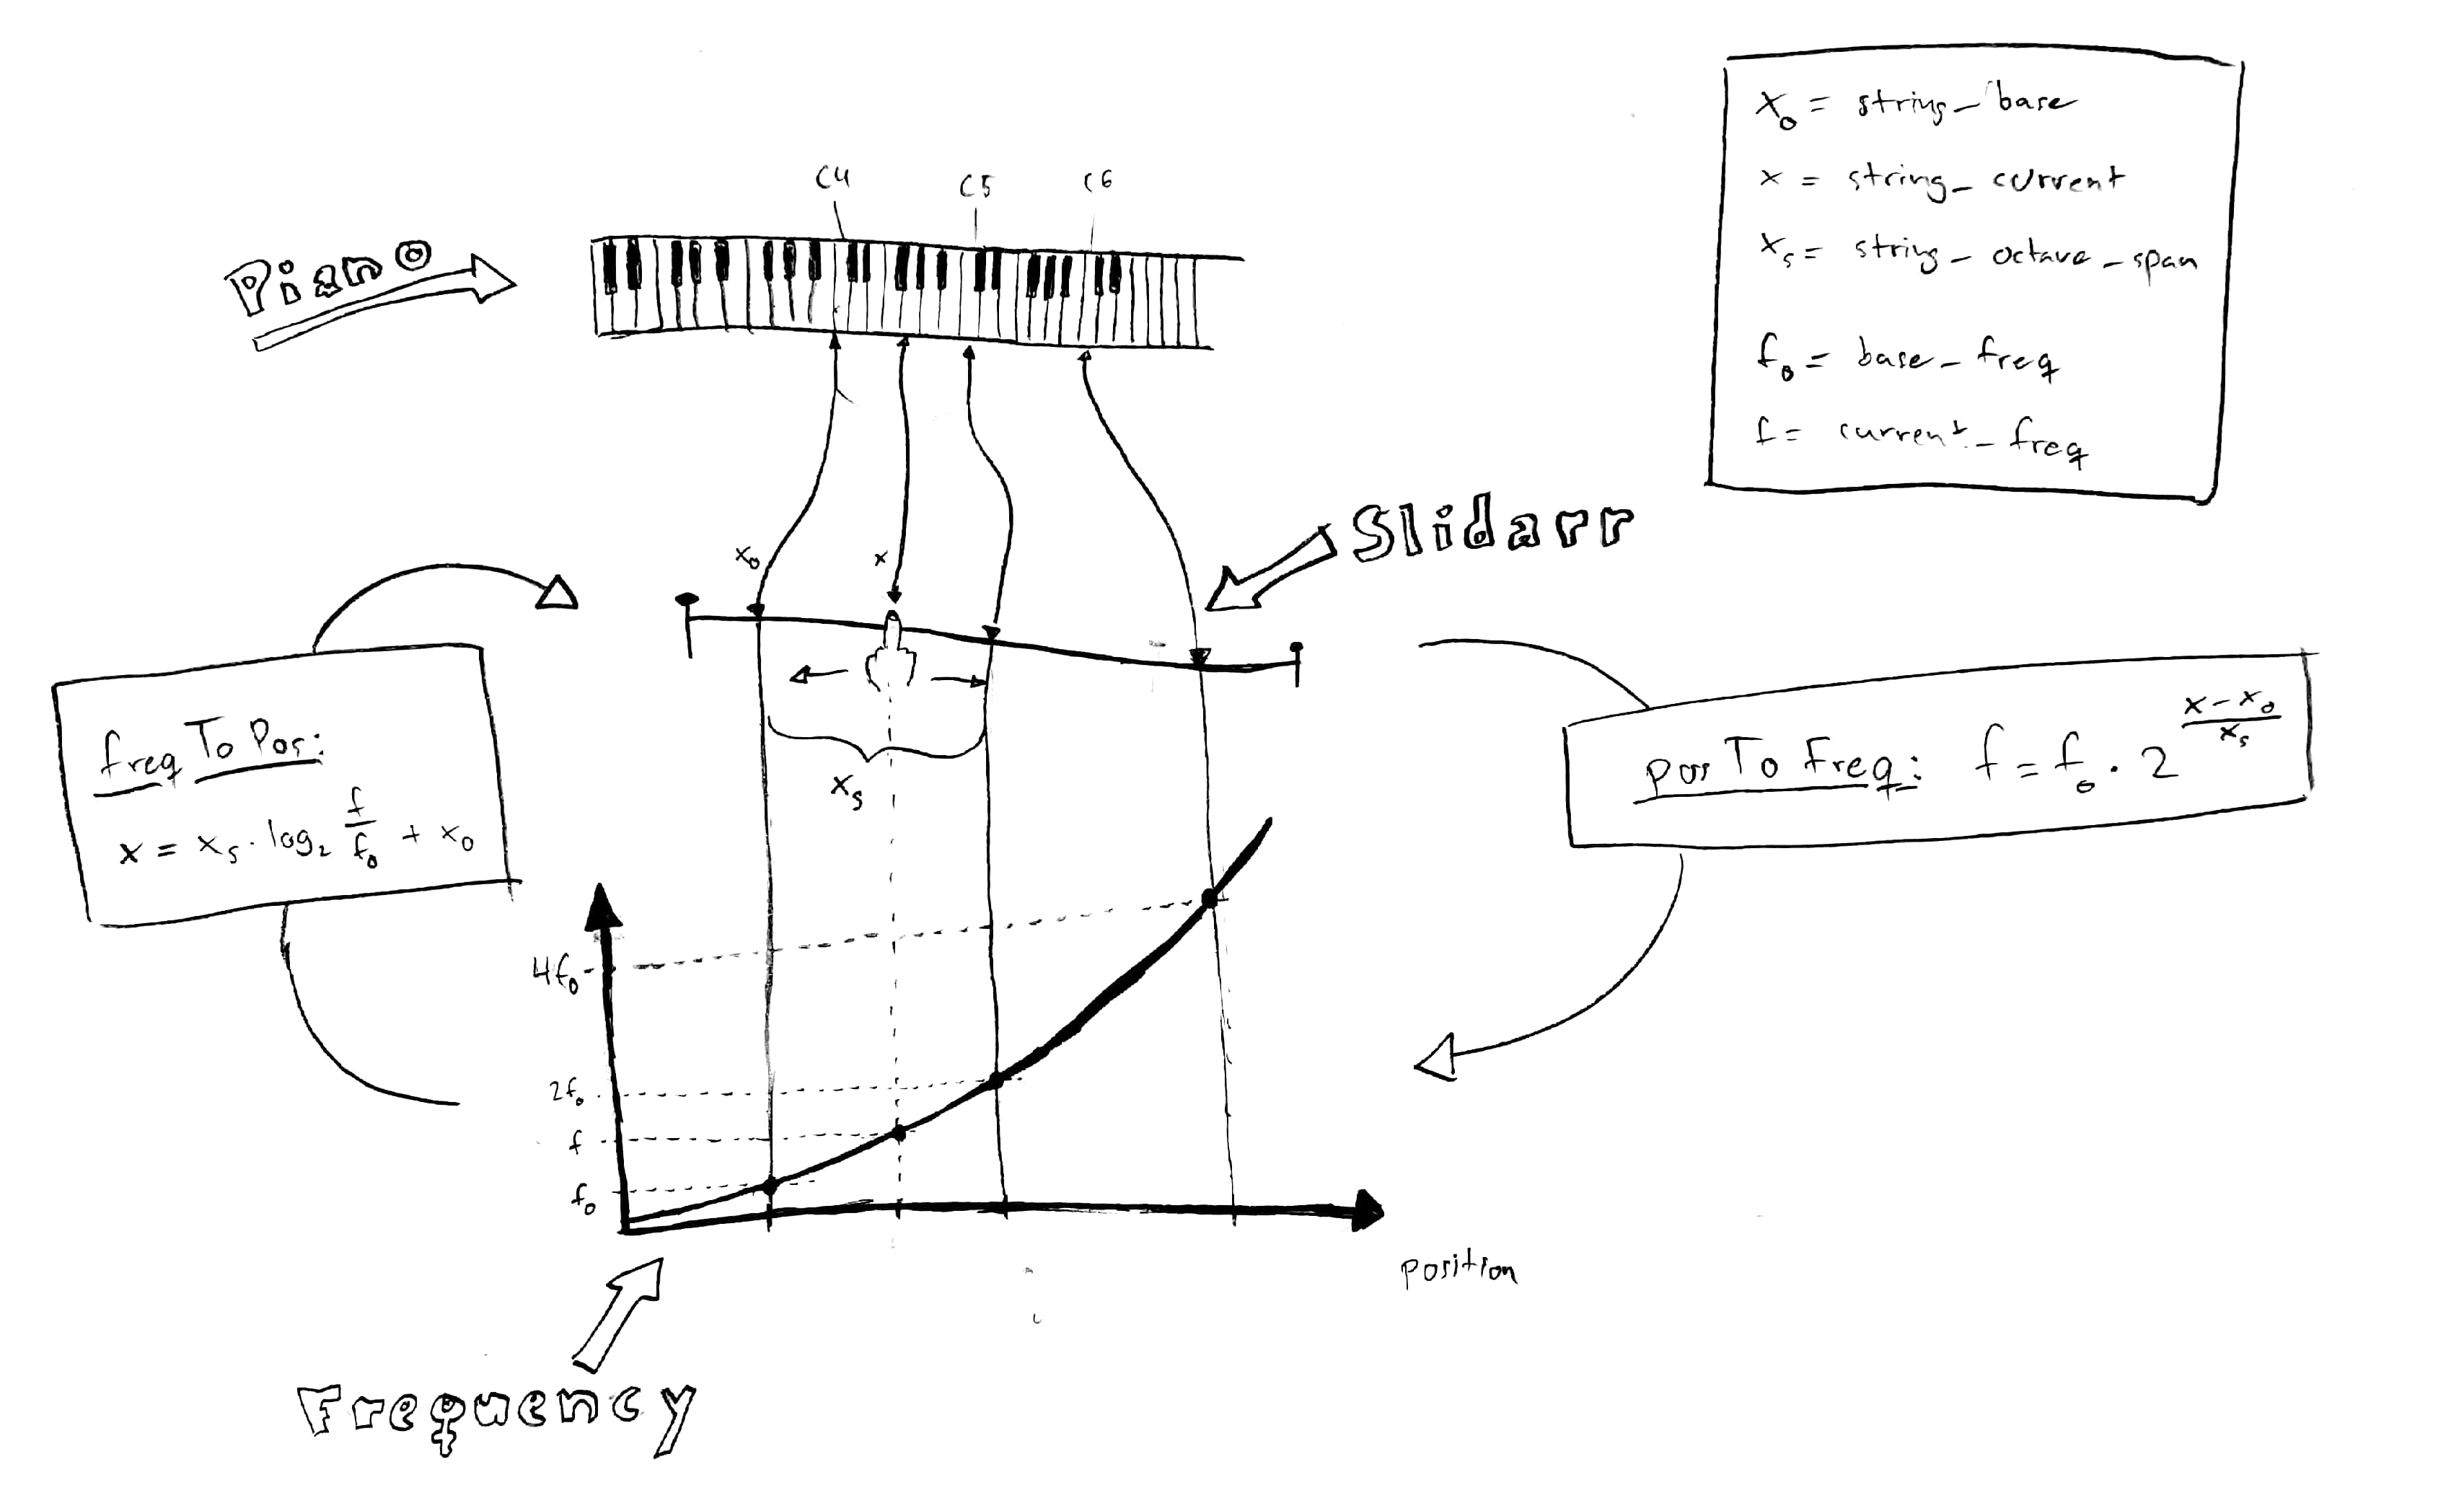
\includegraphics[width=1\textwidth]{slidarr_2_.jpg}
  \caption{slidarr scetch}
  \label{fig:slidarr}
\end{figure}

Blabla blabla bla.

To sum it up these are the major functionalities of the Slidarr and important to know:
\begin{itemize}
 \item Touching, turn specific note on
 \item Sliding, changing the pitch and jumping to another tone
 \item Calibrating, setting the minimum and maximum range on the hardware for one octave
 \item Scrolling, moving the octave on the keyboard to higher or lower tones
\end{itemize}


\section{Analysis}

\subsection{Resistance measurement}
One way of determining the finger's position of the string is to measure the resistance from one end of the string to the finger. A copper wire of length 1 meter and diameter of \SI{0.5}{mm} has a resistance of \SI{0.5}{\ohm} per meter \cite{copperresistance}. In order to track the position  with millimeter accuracy, we need to measure in the sub-\si{\milli\ohm} range. 

This can be done in many different ways. One way is using a resistor bridge setup, e.g. a Wheatstone or Kelvin bridge, which is able to sense tiny changes in resistance. However, the bridge needs to be balanced with accurate resistors of similar value of the measured resistor, which is hard to achieve with standard resistors when the measured resistance is this small.

\begin{figure}[ht]
  \centering
  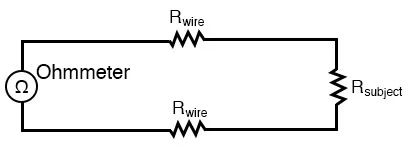
\includegraphics[width=0.5\textwidth]{4-wire-sensing}
  \caption{4-terminal measurement}
  \source{allaboutcircuits.com}
  \label{fig:4terminal}
\end{figure}

An more suitable method is to use four-terminal measurement as shown in figure \ref{fig:4terminal}. A known constant currenti $I$ is fed through the resistor with unknown resistance $R$, and the voltage drop $V$ is measured with a separate pair of wires. The resistance can then easily be calculated using Ohms law, $ R = V / I $.

\subsection{Voltage measurement}
Using four-terminal measurement with a current of \SI{100}{\milli\ampere}, the change in voltage per millimeter string is \SI{50}{\micro\volt}. This has now turned into a matter of measuring low-level voltages.

A 12-bit ADC operating at \SIrange{0}{3.3}{\volt} has a resolution of \SI{0.8}{\milli\volt} per bit. The signal needs to be amplified by at least 16 times in order to achieve \si{\milli\meter} accuracy.

\subsubsection{Instrumentation amplifier}
Since we are interested in the voltage difference over the string, a differential amplifier is a good choice for amplifying the signal. The \textit{instrumentation amplifier} is widely used for amplifying low-level signals. It is stable and easy to adjust, since the amplification can be set by a single resistor \cite{in}.

\subsection{The MIDI protocol}
MIDI (Musical Instrument Digital Interface) protocol is the industry standard for communication between electronic musical instruments and synthesizers \cite{midiorg}. It does not transport the audio itself, instead messages with instructions about the note, its volume and duration are sent to a receiving device which generates the sound. 

MIDI was designed to be used with digital piano keyboards. The messages indicate \textit{note on}, \textit{note off}, and their \textit{velocity} (volume). The protocol is built around the concept of piano notes, which is not optimal for the Slidarr since it operates at a continous scale rather than at fixed frequency intervals.

The solution to this is the \textit{pitchbend} message, which is usually controlled by a wheel controller on the keyboard. It is a global parameter that bends the pitch (offsets the frequency) of the currently played notes, on synths that support it. The amount of bending is not standardized and can differ between synthesizers.

The MIDI message consists of three bytes: the \textit{command} and two \textit{parameters} \cite{midistanford}. There are many different commands, but the Slidarr only needs the three as shown in table \ref{table:midi_msgs}.

\begin{table}[h]
  \centering
  \caption{MIDI messages}
  \label{table:midi_msgs}
  \begin{tabular}{llll}
    Action     & Command & Parameter 1 & Parameter 2 \\ \hline
    Note off   & 0x80    & Key         & Velocity    \\
    Note on    & 0x90    & Key         & Velocity    \\
    Pitch bend & 0xE0    & Value       & Value      
  \end{tabular}
\end{table}

\subsection{Sound generation}
A synthesizer has to be used to generate the sound from the MIDI messages. 

\section{Design}

image of components/blocks here

\subsection{Interface}

\subsection{Electronics}

\section{Implementation}

\subsection{Making MIDI continuous}

\subsection{The state machine}

image of simple state machine

\subsection{Streaming MIDI}

\subsection{Wireless bridge}

\section{Testing and verification}

\section{Results}

\subsection{Feasability}

\subsection{Future improvements and implementations}

picture with concepts


\begin{thebibliography}{9}

\bibitem{copperresistance} 
Chemandy Electronics: Round Wire Resistance Calculator,
\\\texttt{https://chemandy.com/calculators/round-wire-resistance-calculator.htm}

\bibitem{in} 
Electronics Hub: Instrumentation Amplifier Basics and Applications,
\\\texttt{https://www.electronicshub.org/instrumentation-amplifier-basics-applications}

\bibitem{midiorg} 
The MIDI Association,
\\\texttt{https://www.midi.org}

\bibitem{midistanford}
Stanford CCRMA: Essentials of the MIDI protocol,
\\\texttt{https://ccrma.stanford.edu/~craig/articles/linuxmidi/misc/essenmidi.html}

\end{thebibliography}
\end{document}
